
% Copyright (c) 1991-2002, The Numerical ALgorithms Group Ltd.
% All rights reserved.
%
% Redistribution and use in source and binary forms, with or without
% modification, are permitted provided that the following conditions are
% met:
%
%     - Redistributions of source code must retain the above copyright
%       notice, this list of conditions and the following disclaimer.
%
%     - Redistributions in binary form must reproduce the above copyright
%       notice, this list of conditions and the following disclaimer in
%       the documentation and/or other materials provided with the
%       distribution.
%
%     - Neither the name of The Numerical ALgorithms Group Ltd. nor the
%       names of its contributors may be used to endorse or promote products
%       derived from this software without specific prior written permission.
%
% THIS SOFTWARE IS PROVIDED BY THE COPYRIGHT HOLDERS AND CONTRIBUTORS "AS
% IS" AND ANY EXPRESS OR IMPLIED WARRANTIES, INCLUDING, BUT NOT LIMITED
% TO, THE IMPLIED WARRANTIES OF MERCHANTABILITY AND FITNESS FOR A
% PARTICULAR PURPOSE ARE DISCLAIMED. IN NO EVENT SHALL THE COPYRIGHT OWNER
% OR CONTRIBUTORS BE LIABLE FOR ANY DIRECT, INDIRECT, INCIDENTAL, SPECIAL,
% EXEMPLARY, OR CONSEQUENTIAL DAMAGES (INCLUDING, BUT NOT LIMITED TO,
% PROCUREMENT OF SUBSTITUTE GOODS OR SERVICES-- LOSS OF USE, DATA, OR
% PROFITS-- OR BUSINESS INTERRUPTION) HOWEVER CAUSED AND ON ANY THEORY OF
% LIABILITY, WHETHER IN CONTRACT, STRICT LIABILITY, OR TORT (INCLUDING
% NEGLIGENCE OR OTHERWISE) ARISING IN ANY WAY OUT OF THE USE OF THIS
% SOFTWARE, EVEN IF ADVISED OF THE POSSIBILITY OF SUCH DAMAGE.

% *********************************************************************
\head{schapter}{A Technical Introduction to \Language{}}{ugTechIntro}
% *********************************************************************

\Language{} has both
an {\it interactive
language} for user interactions and a
{\it programming language} for building library modules.
Like Modula 2,
\index{Modula 2}
PASCAL,
\index{PASCAL}
FORTRAN,
\index{FORTRAN}
and Ada,
\index{Ada}
the programming language emphasizes strict type-checking.
Unlike these languages, types in \Language{} are dynamic
objects: they are created at run-time in response to user
commands.

Here is the idea of the \Language{} programming language in a nutshell.
\Language{} types range from
algebraic ones (like polynomials,
matrices, and power series) to data structures (like
lists, dictionaries, and input files).
Types combine in any meaningful way.
You can build
polynomials of matrices, matrices of polynomials of
power series, hash tables with symbolic keys and rational function entries,
and so on.

{\it Categories} define
algebraic properties to ensure mathematical
correctness. They ensure, for example,
that matrices of polynomials are OK, but
matrices of input files are not.
Through categories, programs can
discover that polynomials of continued fractions
have a commutative
multiplication whereas polynomials of matrices do not.

Categories allow algorithms to be defined in their most natural
setting. For example,
an algorithm can be defined to solve polynomial
equations over {\it any} field.
Likewise a greatest common divisor
can compute the ``gcd'' of two elements
from {\it any} Euclidean domain.
Categories foil
attempts to compute meaningless ``gcds'', for example, of two hashtables.
Categories also enable
algorithms to be compiled into machine code that can be run with
arbitrary types.

The \Language{} interactive language is oriented towards
ease-of-use.
The \Language{} interpreter uses
type-inferencing to deduce the
type of an object from user input.
Type declarations can generally be omitted for common types in the
interactive language.

So much for the nutshell.
Here are these basic ideas described by ten design principles:

%
%------------------------------------------------------------------------------
\pseudoSection{Types are Defined by Abstract Datatype Programs}
%------------------------------------------------------------------------------

\par %\noindent
Basic types are called {\it domains of computation}, or,
simply, {\it domains.}
\index{domain}
Domains are defined by \Language{} programs of the form:

\begin{verbatim}
Name(...): Exports == Implementation
\end{verbatim}
Each domain has a capitalized {\tt Name} that is
used to refer to the class of its
members.
For example, \spadtype{Integer} denotes ``the class of integers,''
\spadtype{Float}, ``the class of floating point numbers,'' and
\spadtype{String}, ``the class of strings.''

The ``{\tt ...}'' part following {\tt Name} lists zero or more parameters
to the constructor.
Some basic ones like \spadtype{Integer}
take no parameters.
% maybe want to say something about Integer vs. Integer()?
Others, like \spadtype{Matrix}, \spadtype{Polynomial} and
\spadtype{List}, take a single parameter that again must be a domain.
For example, \spadtype{Matrix(Integer)} denotes ``matrices over the
integers,'' \spadtype{Polynomial (Float)} denotes ``polynomial with
floating point coefficients,'' and
\spadtype{List (Matrix (Polynomial (Integer)))} denotes ``lists of matrices
of polynomials over the integers.''
There is no restriction on the number or type of
parameters of a domain constructor.
% give examples with data, SquareMatrix(2, Integer). Point is, args can
% be domains or data

The {\tt Exports} part specifies operations for creating and manipulating
objects of the domain.
For example, type \spadtype{Integer} exports constants
\spad{0} and \spad{1}, and operations
\spadopFrom{+}{Integer}, \spadopFrom{-}{Integer}, and
\spadopFrom{*}{Integer}.
While these operations are common, others such as
\spadfunFrom{odd?}{Integer} and \spadfunFrom{bit?}{Integer} are not.

The {\tt Implementation} part defines functions that
implement the exported operations of the domain.
These functions are frequently described in terms of another
lower-level domain used to represent the objects of the domain.

\newpage
%------------------------------------------------------------------------------
\pseudoSection{The Type of Basic Objects is a Domain or Subdomain}
%------------------------------------------------------------------------------

\par %\noindent
Every \Language{} object belongs to a {\it unique} domain.
The domain of an object is also called its {\it type.}
Thus the integer \spad{7} has type \spad{Integer} and the string {\tt
"daniel"} has type \spad{String}.

The type of an object, however, is not unique.
The type of integer \spad{7} is not only \spadtype{Integer}
but \spad{NonNegativeInteger}, \spad{PositiveInteger}, and
possibly, in general, any other
``subdomain'' of the domain \spad{Integer}.
A {\it subdomain}
\index{subdomain}
is a domain with a ``membership predicate''.
\spad{PositiveInteger} is a subdomain of \spad{Integer} with the
predicate ``is the integer \spad{> 0}?''.

Subdomains with names are defined by
abstract datatype programs similar to those for domains.
The {\it Export} part of a subdomain, however, must
list a subset of the exports of the domain.
The {\tt Implementation} part optionally gives special
definitions for subdomain objects.

%------------------------------------------------------------------------------
\pseudoSection{Domains Have Types Called Categories}
%------------------------------------------------------------------------------

\par %\noindent
Domain and subdomains in \Language{} are themselves objects
that have types.
The type of a domain or subdomain is called a {\it category}.
\index{category}
Categories are described by programs of the form:

\begin{verbatim}
Name(...): Category == Exports
\end{verbatim}
The type of every category is the distinguished symbol {\tt Category.}
The category {\tt Name} is used to designate the class of domains of that
type.
For example, category \spadtype{Ring} designates the class of all rings.
Like domains, categories can take zero or more parameters as indicated by the
``{\tt ...}'' part following {\tt Name.}
Two examples are \spadtype{Module(R)} and \spadtype{MatrixCategory(R,Row,Col)}.

The {\tt Exports} part defines a set of operations.
For example, \spadtype{Ring} exports the operations
\spadopFrom{0}{Ring}, \spadopFrom{1}{Ring},
\spadopFrom{+}{Ring}, \spadopFrom{-}{Ring}, and \spadopFrom{*}{Ring}.
Many algebraic domains such as
\spadtype{Integer} and \spadtype{Polynomial (Float)} are rings.
\spadtype{String} and \spadtype{List (R)} (for any domain
\spad{R}) are not.

Categories serve to ensure the type-correctness.
The definition of matrices states {\tt Matrix(R:
Ring)} requiring its single parameter \spad{R} to be a ring.
Thus a ``matrix of polynomials'' is allowed, but
``matrix of lists'' is not.

%Unlike domains, categories say nothing about representation and
%thus serve as abstractions of domains.

%------------------------------------------------------------------------------
\pseudoSection{Operations Can Refer To Abstract Types}
%------------------------------------------------------------------------------

\par %\noindent
All operations have prescribed source and target types.
Types can be denoted by symbols that stand for domains, called
``symbolic domains.''
The following lines of \Language{} code use a symbolic domain \spad{R}:

\begin{verbatim}
R: Ring
power: (R, NonNegativeInteger): R -> R
power(x, n) == x ** n
\end{verbatim}

Line 1 declares the symbol \spad{R} to be a ring.
Line 2 declares the type of \spad{power} in terms of \spad{R}.
From the definition on line 3, \spad{power(3,2)} produces 9 for
\spad{x = 3} and
\spad{R =} \spadtype{Integer}.
Also, \spad{power(3.0,2)} produces \spad{9.0} for
\spad{x = 3.0} and \spad{R =} \spadtype{Float}.
\spad{power("oxford",2)} however fails since \spad{"oxford"} has
type \spadtype{String} which is not a ring.

Using symbolic domains, algorithms can be defined in their most
natural or general setting.

%------------------------------------------------------------------------------
\pseudoSection{Categories Form Hierarchies}
%------------------------------------------------------------------------------

\par %\noindent
Categories form hierarchies (technically, directed-acyclic graphs).
A simplified hierarchical world of algebraic categories is shown below in
Figure \texht{\ref{fig:techintro-1}}{1}.
At the top of this world is \spadtype{SetCategory},
the class of algebraic sets.
The notions of parents, ancestors, and descendants
is clear.
Thus ordered sets (domains of category \spadtype{OrderedSet}) and rings
are also algebraic sets.
Likewise, fields and integral domains are rings and algebraic sets.
However fields and integral domains are not ordered sets.

\begin{texonly}
\vskip .5\baselineskip
%\horizontalline
\begin{figure}[htbp]
  \begin{center}
    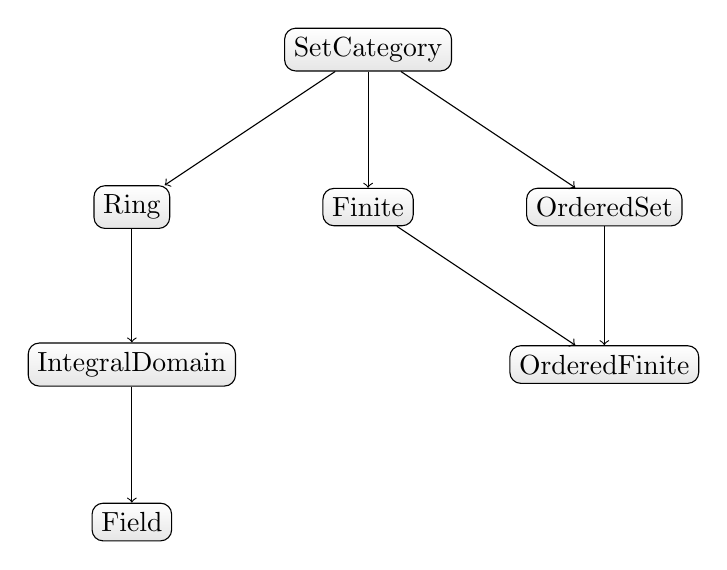
\begin{tikzpicture}[every node/.style = {shape=rectangle, rounded corners,
        draw, align=center, top color=white, bottom color=gray!20}]]
      \node(SetCategory) at (3,6) {\spadtype{SetCategory}};
      \node(Ring) at (0,4) {\spadtype{Ring}};
      \node(IntegralDomain) at (0,2) {\spadtype{IntegralDomain}};
      \node(Field) at (0,0) {\spadtype{Field}};
      \node(Finite) at (3,4) {\spadtype{Finite}};
      \node(OrderedSet) at (6,4) {\spadtype{OrderedSet}};
      \node(OrderedFinite) at (6,2) {\spadtype{OrderedFinite}};

      \draw[->](SetCategory)--(Ring);
      \draw[->]               (Ring)--(IntegralDomain);
      \draw[->]                       (IntegralDomain)--(Field);

      \draw[->](SetCategory)--(Finite);
      \draw[->]               (Finite)--(OrderedFinite);

      \draw[->](SetCategory)--(OrderedSet);
      \draw[->]               (OrderedSet)--(OrderedFinite);
    \end{tikzpicture}
  \end{center}
  \caption{A simplified category hierarchy.\label{fig:techintro-1}}
\end{figure}
%\horizontalline
\vskip .5\baselineskip
\end{texonly}
\begin{htonly}
\beginImportant
\begin{verbatim}
SetCategory +---- Ring       ---- IntegralDomain ---- Field
            |
            +---- Finite     ---+
            |                    \
            +---- OrderedSet -----+ OrderedFinite
\end{verbatim}
\begin{center}
Figure 1.  A  simplified category hierarchy.
\end{center}
\endImportant
\end{htonly}


\newpage

%------------------------------------------------------------------------------
\pseudoSection{Domains Belong to Categories by Assertion}
%------------------------------------------------------------------------------

\par %\noindent
A category designates a class of domains.
Which domains?
You might think that \spadtype{Ring} designates the class of all
domains that export
\spad{0}, \spad{1},
\spadopFrom{+}{Integer}, \spadopFrom{-}{Integer}, and
\spadopFrom{*}{Integer}.
But this is not so.
Each domain must {\it assert} which categories it belongs to.

The {\tt Export} part of the definition for \spadtype{Integer}
reads, for example:

\begin{verbatim}
Join(OrderedSet, IntegralDomain,  ...) with ...
\end{verbatim}
This definition asserts that \spadtype{Integer} is
both an ordered set and an integral domain.
In fact, \spadtype{Integer} does not explicitly export constants
\spad{0} and \spad{1} and operations \spadopFrom{+}{Ring},
\spadopFrom{-}{Ring} and
\spadopFrom{*}{Ring} at all: it inherits them all from \spad{Ring}!
Since \spadtype{IntegralDomain} is a descendant of \spad{Ring},
\spadtype{Integer} is therefore also a ring.

Assertions can be conditional.
For example, \spadtype{Complex(R)} defines its exports by:

\begin{verbatim}
Ring with ... if R has Field then Field ...
\end{verbatim}
Thus \spadtype{Complex(Float)} is a field but \spadtype{Complex(Integer)}
is not since \spadtype{Integer} is not a field.

You may wonder:
``Why not simply let the set of operations determine
whether a domain belongs to a given category?''.
\Language{} allows operation names (for example,
\spadfun{norm}) to have very different
meanings in different contexts.
The meaning of an operation in \Language{} is determined by context.
By associating operations with categories, operation names can be reused
whenever appropriate or convenient to do so.
As a simple example, the operation \spadop{<} might be used to denote
lexicographic-comparison in an algorithm.
However, it is wrong to use the same \spadop{<} with this
definition of absolute-value: {\tt abs(x) == if x < 0 then -x
else x.}
Such a definition for {\tt abs} in \Language{} is protected by context:
argument \spad{x} is required to be a
member of a domain of category \spadtype{OrderedSet}.

%------------------------------------------------------------------------------
\pseudoSection{Packages Are Clusters of Polymorphic Operations}
%------------------------------------------------------------------------------

\par %\noindent
In \Language{}, facilities for symbolic integration, solution of equations, and the like
are placed in ``packages''.
A {\it package}
\index{package}
is a special kind of domain: one whose exported operations
depend solely on the parameters of the constructor and/or
explicit domains.

If you want to use \Language{}, for example, to define some algorithms for solving
equations of polynomials over an arbitrary field \spad{F}, you
can do so with a package of the form:

\begin{verbatim}
MySolve(F: Field): Exports == Implementation
\end{verbatim}

where {\tt Exports} specifies the \spadfun{solve} operations you wish to
export and {\tt Implementation} defines functions for implementing your algorithms.
Once \Language{} has compiled your package, your algorithms can then be used
for any \spad{F}: floating-point numbers, rational numbers, complex
rational functions, and power series, to name a few.

% I think you need to talk somewhere about function implementations.
% You can also mention alternative implementations based on "has"
% conditionals.

%------------------------------------------------------------------------------
\pseudoSection{The Interpreter Builds Domains Dynamically}
%------------------------------------------------------------------------------

\par %\noindent
The \Language{} interpreter reads user input then builds whatever types
it needs to perform the indicated computations.
For example, to create the matrix
\begin{texonly}
\[M = \begin{pmatrix}x^2+1&0\\0&x / 2\end{pmatrix}\]
\end{texonly}
\begin{htonly}
\spad{M = [[x^2+1,0],[0,x / 2]]}
\end{htonly}
the interpreter first loads the
modules \spadtype{Matrix}, \spadtype{Polynomial}, \spadtype{Fraction},
and \spadtype{Integer} from the library, then builds the {\it domain tower}
``matrices of polynomials of rational numbers (fractions of integers)''.
% also, categories get loaded plus auxiliary domains
%\footnote{Most systems are preloaded with such common types; once
%modules are loaded they are immediately available to the interpreter.}

Once a domain tower is built, computation proceeds by calling operations
down the tower.
% "down the tower" is confusing
For example, suppose that the user asks to square the above matrix.
To do this, the function \spadopFrom{*}{Matrix} from \spadtype{Matrix}
is passed \spad{M} to compute \spad{M * M}.
The function is also passed
an environment containing \spad{R} that, in this case, is
\spadtype{Polynomial (Fraction (Integer))}.
This results in the successive calling of the \spadopFrom{*}{Fraction}
operations from \spadtype{Polynomial}, then from \spadtype{Fraction}, and
then finally from \spadtype{Integer} before a result is passed back up
the tower.

Categories play a policing role in the building of domains.
Because the argument of \spadtype{Matrix} is required to be
a ring, \Language{} will not build nonsensical types such as
``matrices of input files''.

%------------------------------------------------------------------------------
\pseudoSection{\Language{} Code is Compiled}
%------------------------------------------------------------------------------

\par %\noindent
\Language{} programs are statically compiled to machine code,
then placed into library modules.
Categories provide an important role in obtaining efficient object code by enabling:
\begin{itemize}
\item static type-checking at compile time;
\item fast linkage to operations in domain-valued parameters;
\item optimization techniques to be used for partially specified types
(operations for ``vectors of \spad{R}'', for instance, can be open-coded even
though \spad{R} is unknown).
\end{itemize}

%------------------------------------------------------------------------------
\pseudoSection{\Language{} is Extensible}
%------------------------------------------------------------------------------

\par %\noindent
Users and system implementers alike use the \Language{} language
to add facilities to the \Language{} library.
The entire \Language{} library is in fact written in the \Language{}
source code and available for user modification and/or extension.

\Language{}'s use of abstract datatypes clearly separates the exports
of a domain (what operations are defined) from its implementation (how
the objects are represented and operations are defined).
Users of a domain can thus only create and manipulate objects through
these exported  operations.
This allows implementers to ``remove and replace''
parts of the library safely by newly upgraded (and, we hope, correct)
implementations without consequence to its users.

Categories protect names by context,
making the same names available for use in other contexts.
Categories also provide for code-economy.
Algorithms can be parameterized categorically
to characterize their correct and most general context.
Once compiled, the same machine code is applicable
in all such contexts.

Finally, \Language{} provides an automatic, guaranteed interaction between
new and old code.
For example:
\begin{itemize}
\item if you write a new algorithm that requires a parameter to be a
field, then your algorithm will work automatically with every field
defined in the system; past, present, or future.
\item if you introduce a new domain constructor that produces a field,
then the objects of that domain can be used as parameters to any algorithm
using field objects defined in the system; past, present, or future.
\end{itemize}

These are the key ideas.
For further information, we particularly recommend your reading
chapters 11, 12, and 13, where these ideas are explained
in greater detail.
